\section{Introduction}
%Various areas, including social networks, chemical compounds, graph neural networks, and citation networks, use graphs as their underlying data structure. With the widespread adoption of graphs and the increasing graph size, many algorithms have been proposed to analyze graphs efficiently. Among these algorithms, subgraph search has always played an essential role in graph data mining.
%
%The goal of subgraph search is to find all subgraphs in a data graph $G$ that are isomorphic to a given query graph $q$. Though the problem
%is NP-complete, many approaches
%\cite{bhattarai2019ceci,guo2020gpu,tran2015fast,shi2020graphpi,bi2016efficient,zeng2020gsi,sun2020subgraph,guo2020exploiting,sun2020rapidmatch,lin2016network}
%have been proposed to speed up subgraph search in recent years. All these approaches adopt a similar 3-step procedure. They first build
%candidate sets and auxiliary data for query vertices, then generate a matching order for query vertices based on candidate sets and
%auxiliary data and finally match $q$ in $G$ according to the matching order. Most previous works mainly focus on generating an effective
%matching order that can reduce the number of intermediate results during subgraph search. For example, the main idea of the matching order
%generation algorithm proposed in \cite{bi2016efficient} is to match all non-tree edges regarding any spanning tree of $q$ as soon as
%possible to eliminate invalid subgraph candidates in the early stages of the matching process. We borrow this idea when designing our
%matching order generation algorithm.
%
%Some works \cite{lin2016network,guo2020gpu,tran2015fast,zeng2020gsi,guo2020exploiting} focus on optimizing subgraph search on GPUs, and GSI
%\cite{zeng2020gsi} achieves the best performance among all these approaches. GSI designs an edge label partitioned CSR (PCSR) format for a
%data graph to speed up accessing vertex neighbors. To build a PCSR format for a data graph, GSI first groups edges and corresponding
%vertices by the edge label into edge label partitions. Then, GSI builds a GPU-based CSR format for each edge label partition, which is the
%PCSR format. In order to find the position of a given vertex ID (VID) in PCSR, GSI adopts a hash function to map VIDs to positions
%(hash-PCSR), which needs many empty entries to reduce collisions (GSI uses 30 empty entries for each VID). In our approach, we also utilize
%PCSR format but replace the hash function with interval indexes (interval-PCSR). Additionally, we design a VID mapping algorithm for
%vertices in $G$ to map old VIDs to new VIDs, which can create more contiguous VIDs in each edge label partition and hence reduce the number
%of intervals. GSI proposes a Prealloc-Combine approach to make the parallel write of intermediate results more efficient. Nevertheless,
%this approach needs to launch two extra GPU kernels to write intermediate results to the right place. Unlike GSI, we utilize atomic
%operations inside the GPU kernel to calculate right positions for intermediate results. Therefore, we do not need extra GPU kernels.

Subgraph matching is a fundamental task of graph analysis. It requires finding all subgraphs from a data graph $G$ that are isomorphic to a
query graph $q$. This technique has a wide range of applications, including social network analysis \FIXME{\cite{}}, and chemical compound
search \FIXME{\cite{}}.

Subgraph matching is an NP-complete problem \FIXME{\cite{}}, requiring significant computation time when processing large, real-life
graphs. A wide range of approaches have been proposed to speed up subgraph search
\cite{bhattarai2019ceci,guo2020gpu,tran2015fast,shi2020graphpi,bi2016efficient,zeng2020gsi,sun2020subgraph,guo2020exploiting,sun2020rapidmatch,lin2016network}.
These approaches a typical 3-step process for subgraph matching. From the vertices in the query graph $q$, this process first builds
candidate sets and auxiliary data from the data graph $G$. It then determines a matching order that determines how each query vertice
should be matched from the candidate sets and auxiliary data before performing the graph matching by following the matching order.

Some of the most recent works attempt to leverage the GPU computation power for fast graph matching
\cite{lin2016network,guo2020gpu,tran2015fast,zeng2020gsi,guo2020exploiting}. GSI is the current state-of-the-art GPU-based graph matching
algorithm \cite{zeng2020gsi}, delivering the best performance on some of the representative datasets. It has a dedicated graph storage
format to reduce the memory footprint and improve the performance for graph vertice matching. While promising, exisiting approaches can
only match one vertice from the query graph in one go. Such a strategy leads to extensive GPU memory accesses because they need to load and
store the intermediate results for each vertice matching. These memory operations are expensive on GPUs with sizeable intermediate results.



All the abovementioned works match vertices of $q$ one by one, and thus need to write the intermediate results after matching one vertex
and read the same intermediate results before matching the next vertex. The write and read operations are time-consuming, especially when
the size of intermediate results is significant. To mitigate the cost of write and read operations, Lai et al. \cite{lai2015scalable}
utilize MapReduce to implement a double-edge extension method. Their approach iteratively matches the query graph by a TwinTwig that
consists of one edge (matching pattern 0 in Figure \ref{fig:matchpattern}) or two incident edges of a vertex (matching patterns 1 and 3 in
Figure \ref{fig:matchpattern}). However, there are three inherent limitations in \cite{lai2015scalable}. First, edges in a TwinTwig must
grow from the same vertex, which means their approach can not handle matching patterns 2, 4, and 7 in Figure \ref{fig:matchpattern}.
Second, a TwinTwig contains at most two edges, but more than two edges can be processed at the same time, like matching patterns 5 and 6.
Third, they use a simple method to generate results for matching pattern 1, which causes a number of unnecessary memory accesses to
neighbors.

To overcome limitations of \cite{lai2015scalable}, we propose an approach that performs subGraph sEarch usiNg parallEl Vertex mAtching (\SystemName).  Specifically, \SystemName matches as many query vertices as possible at each iteration and generate corresponding results in one GPU kernel. First, our approach can match vertices from different source vertices, e.g., matching patterns 2 and 4. Second, our approach can match as many edges as possible in a single GPU kernel (illustrated in Section \ref{sec:eliphase}). Third, we design an optimized algorithm (Algorithm \ref{algo:optDV}) to reduce unnecessary memory accesses for matching pattern 1. Moreover, we develop a new matching order generation algorithm (Algorithm \ref{algo:genmatchorder}) that is designed specifically for \SystemName. In summary, our approach can handle all matching patterns in Figure \ref{fig:matchpattern}.

\begin{figure}
\centering
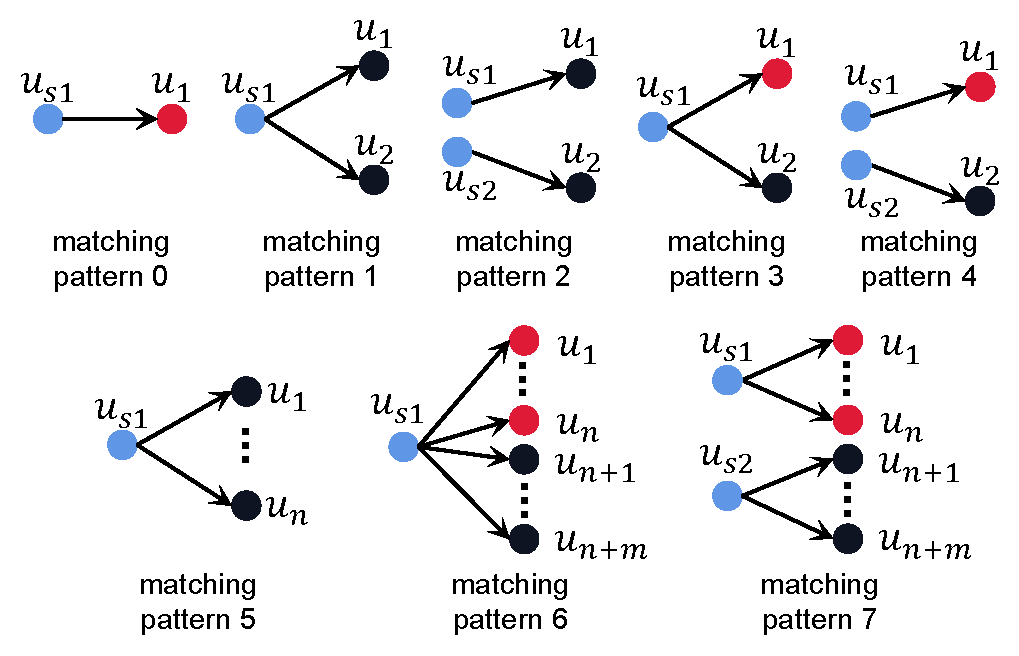
\includegraphics[width=0.9\columnwidth]{./figure/extpattern.eps}
\caption{Matching patterns supported by \SystemName. $u_{s1}$ and $u_{s2}$ represent matched query vertices, and can be any vertex labels. \{$u_1, \cdots, u_{n}$\} and
\{$u_{n+1}, \cdots, u_{n+m}$\} represent query vertices to be matched, and vertices in the same set have the same vertex label. Edges in the the same matching pattern have the same edge label.}
\label{fig:matchpattern}
\end{figure}

 We validate our approach from three aspects: (1) Experimental results show that our interval-PCSR significantly reduces the space cost and searching time of hash-PCSR by 83\% and 58\% respectively; (2) We obtain an average speedup of $5\times$ over GSI for subgraph search; (3) Compared to the single vertex matching , which is modified based on our parallel vertex matching, our approach reduces the search time by 15.9\% on average.

 To summarize, we make the following contributions:
 \begin{itemize}
  \item We propose an interval-PCSR format and a mapping algorithm that can generate more contiguous VIDs in each edge label partition. Our interval-PCSR significantly reduces the space cost and searching time of hash-PCSR of GSI.
  \item We propose a parallel vertex matching method that can match as many query vertices as possible to reduce the number of read and write operations of intermediate results.
  \item We propose a new matching order generation algorithm and a new parallel write scheme to accommodate \SystemName.
\end{itemize}
